This internship is carried out within the scope of the SEAWINGS and AIRSHIP projects, initiatives aimed at developing innovative autonomous aerial platforms specifically designed to operate over maritime environments. The distinguishing feature of these platforms is their design as Wing-In-Ground (WIG) effect vehicles. These vehicles stand out for the operational requirement of flying at high speeds and extremely low altitudes, often only one or two metres above the water surface. This flight configuration takes advantage of the aerodynamic "ground effect" phenomenon, creating a cushion of air beneath the structure that drastically increases the vehicle's lift and energy efficiency.

\begin{figure}[h]
     \centering
          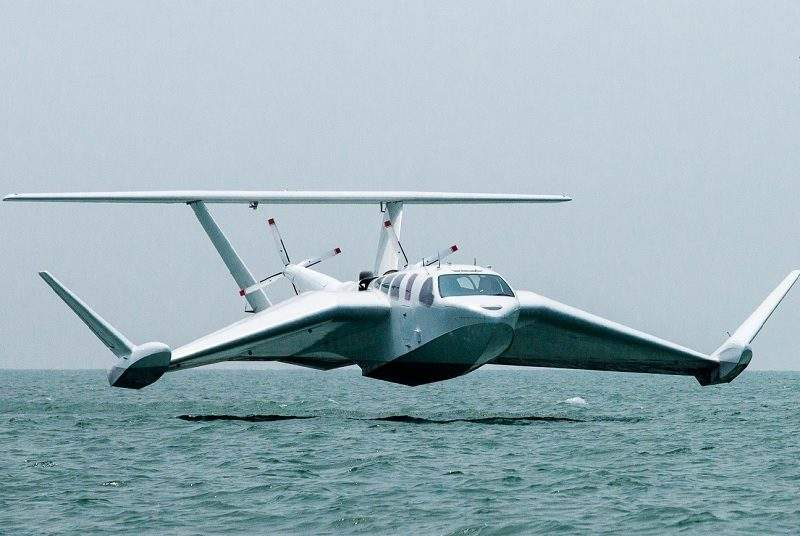
\includegraphics[width=0.7\textwidth]{../imagens/wig.jpg}
     \caption{Example of a vehicle operating under the Wing-In-Ground (WIG) effect principle.}
     \label{fig:wig_effect}
 \end{figure}

Because of this requirement for fast, low-altitude flight, one of the central and most critical challenges of these projects is accurate, real-time perception of the sea surface. In an environment where the margin for error is minimal and the fluid dynamics are unpredictable, timely detection of waves is not merely a matter of topographic mapping, but a fundamental safety requirement. The ability to "see" the water ahead of the vehicle ensures that the control systems can perform evasive manoeuvres or altitude adjustments, avoiding catastrophic collisions with the swell.

Ocean waves are a dynamic and periodic phenomenon, characterized mainly by their amplitude, direction and frequency. Correctly estimating the geometric and kinematic values of these parameters, as well as the ability to predict the short-term temporal and spatial propagation of waves, contributes significantly to the robustness of the control and trajectory-planning systems of these platforms under development.
